\documentclass[12pt]{article}

\usepackage{fourier}
\usepackage{amsmath}
\usepackage{siunitx}
\usepackage{bm}
\usepackage{color}
\usepackage{graphicx,url}
\usepackage{float}
\usepackage{amsfonts,amsmath,bm,bbm}
\usepackage{booktabs}
\usepackage{multicol,multirow}

\title{Experiments with Confidence Regions}
\author{}
\date{}

\begin{document}

\section{Experiment \#1}

\begin{description}
	\item[Purpose:] study the effect of injecting correlation on the emblematic time series
	\item[Setup:]\mbox{} 
		\begin{itemize}
			\item the emblematic series $\bm x$ of size $N=\num{10000}$ whose point in the $H\times C$ plane, say $\big(h, c\big)(\bm x)$, is the median point of the first principal component.
			\item the confidence regions at the \SI{95}{\percent} and \SI{99}{\percent} for $\bm x$
		\end{itemize}
	\item[Experiment:] \mbox{}
		\begin{enumerate}
			\item Draw the confidence regions.
			\item Draw $\big(h,c\big)(\bm x)$.
			\item Define the parameter grid $k\in\{0,\Delta k, 2\Delta k,\dots, k_{\max}\}$.
			\item For each value of $k$, compute $\widetilde{\bm x}^{(k)}$, the series obtained by introducing power spectrum of order $1/k$ in $\bm x$.
			\item Compute and draw $\big(h,c\big)(\widetilde{\bm x}^{(k)})$.
			\item Analyze the values of $k$ for which these points are inside the confidence regions, and the smallest one for which $\big(h,c\big)(\widetilde{\bm x}^{(k)})$ is outside them.
		\end{enumerate}
	
	\begin{figure}[H]
		\includegraphics[width=\linewidth]{../../Images/Correlation-Analysis.pdf}
	\end{figure}
\end{description}

\section{Experiment \#2}

\begin{description}
	\item[Purpose:] study the effect of injecting a deterministic component to the emblematic time series
	\item[Setup:]\mbox{} 
	\begin{itemize}
		\item the emblematic series $\bm x$ of size $N=\num{10000}$ whose point in the $H\times C$ plane, say $\big(h, c\big)(\bm x)$, is the median point of the first principal component.
		\item the sine function $\bm x'=\big(\sin(2x) \big)_{1\leq i\leq N}$.
		\item the confidence regions at the \SI{95}{\percent} and \SI{99}{\percent} for $\bm x$
	\end{itemize}
	\item[Experiment:] \mbox{}
	\begin{enumerate}
		\item Draw the confidence regions.
		\item Draw $\big(h,c\big)(\bm x)$.
		\item Define the parameter grid $\alpha\in\{0,\Delta \alpha, 2\Delta \alpha,\dots, \alpha_{\max} = 1\}$
		\item For each value of $\alpha$ compute the time series $\widetilde{\bm x}^{(\alpha)}=\alpha\bm x + (1-\alpha)\bm x'$.
		\item Compute and draw $\big(h,c\big)(\widetilde{\bm x}^{(\alpha)})$.
		\item Analyze the values of $\alpha$ for which these points are inside the confidence regions, and the smallest one for which $\big(h,c\big)(\widetilde{\bm x}^{(\alpha)})$ is outside them.
	\end{enumerate}
	
	\begin{figure}[H]
	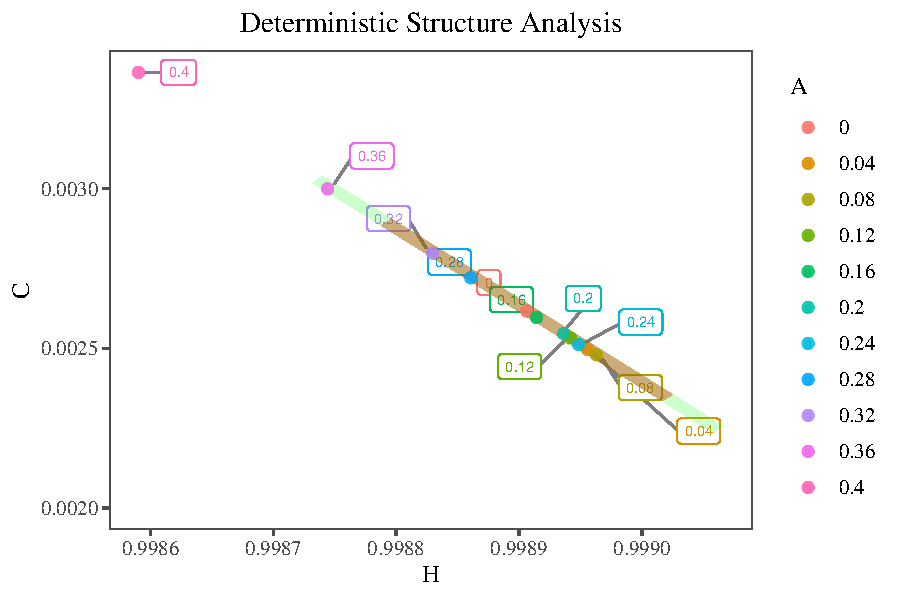
\includegraphics[width=\linewidth]{../../Images/Deterministic-Analysis.pdf}
	\end{figure}

\end{description}

\newpage

\section{Experiment \#3}

\begin{description}
	\item[Purpose:] assess the quality of sequences produced by the \texttt{PRNG} algorithm
	\item[Setup:]\mbox{} 
	\begin{itemize}
		\item $100$ non-overlapping series of size $N$ produced by \texttt{PRNG}
		\item the confidence regions at the \SI{95}{\percent} and \SI{99}{\percent} for $\bm x$
	\end{itemize}
	\item[Experiment:] \mbox{}
	\begin{enumerate}
		\item Draw the confidence regions.
		\item Compute and draw $\big(h,c\big)$ for each of the $100$ series produced by \texttt{PRNG}
		\item Count how many fall inside/outside the regions.
	\end{enumerate}
	
	\begin{figure}[H]
	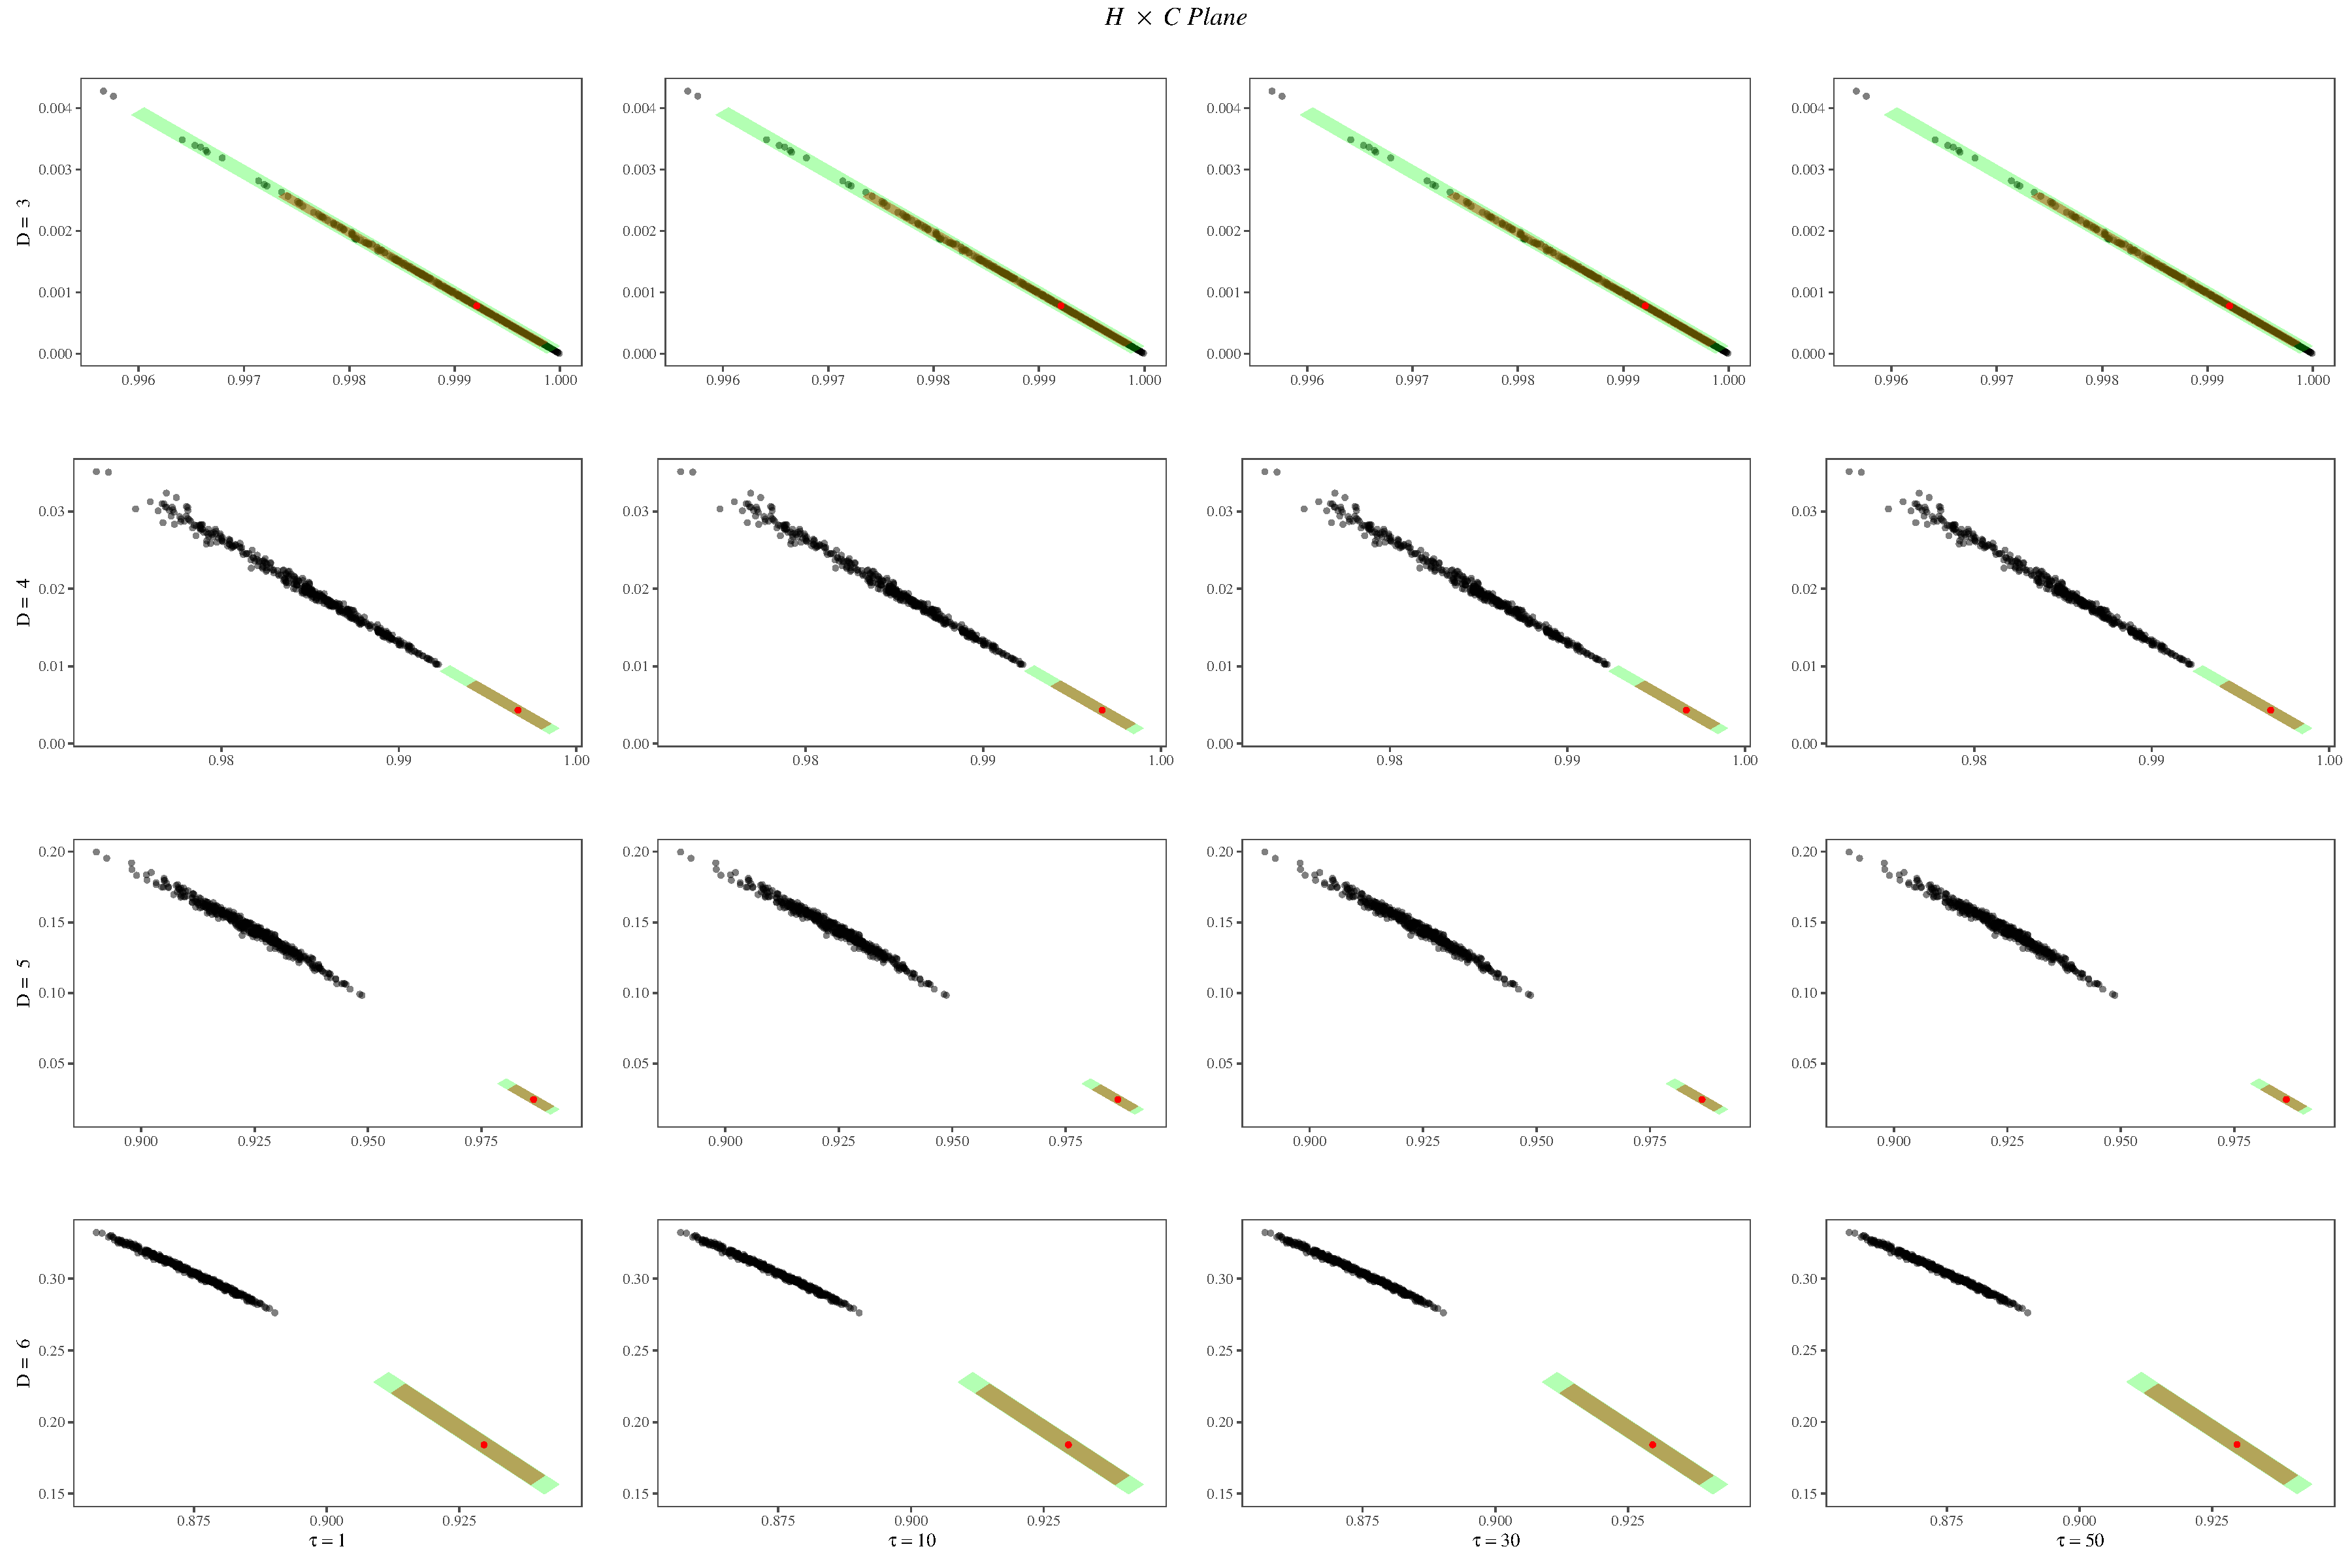
\includegraphics[width=\linewidth]{../../Images/PRNGs/N1000/Mersenne-1000.pdf}
	\caption{Scatter diagrams of the Mersenne-Twister sequences with 1.000 observations for D $\in \{3,4,5,6\}$ (columns) and $\tau \in \{1,10,30,50\}$ (lines).}
	\end{figure}

	\begin{figure}[H]
	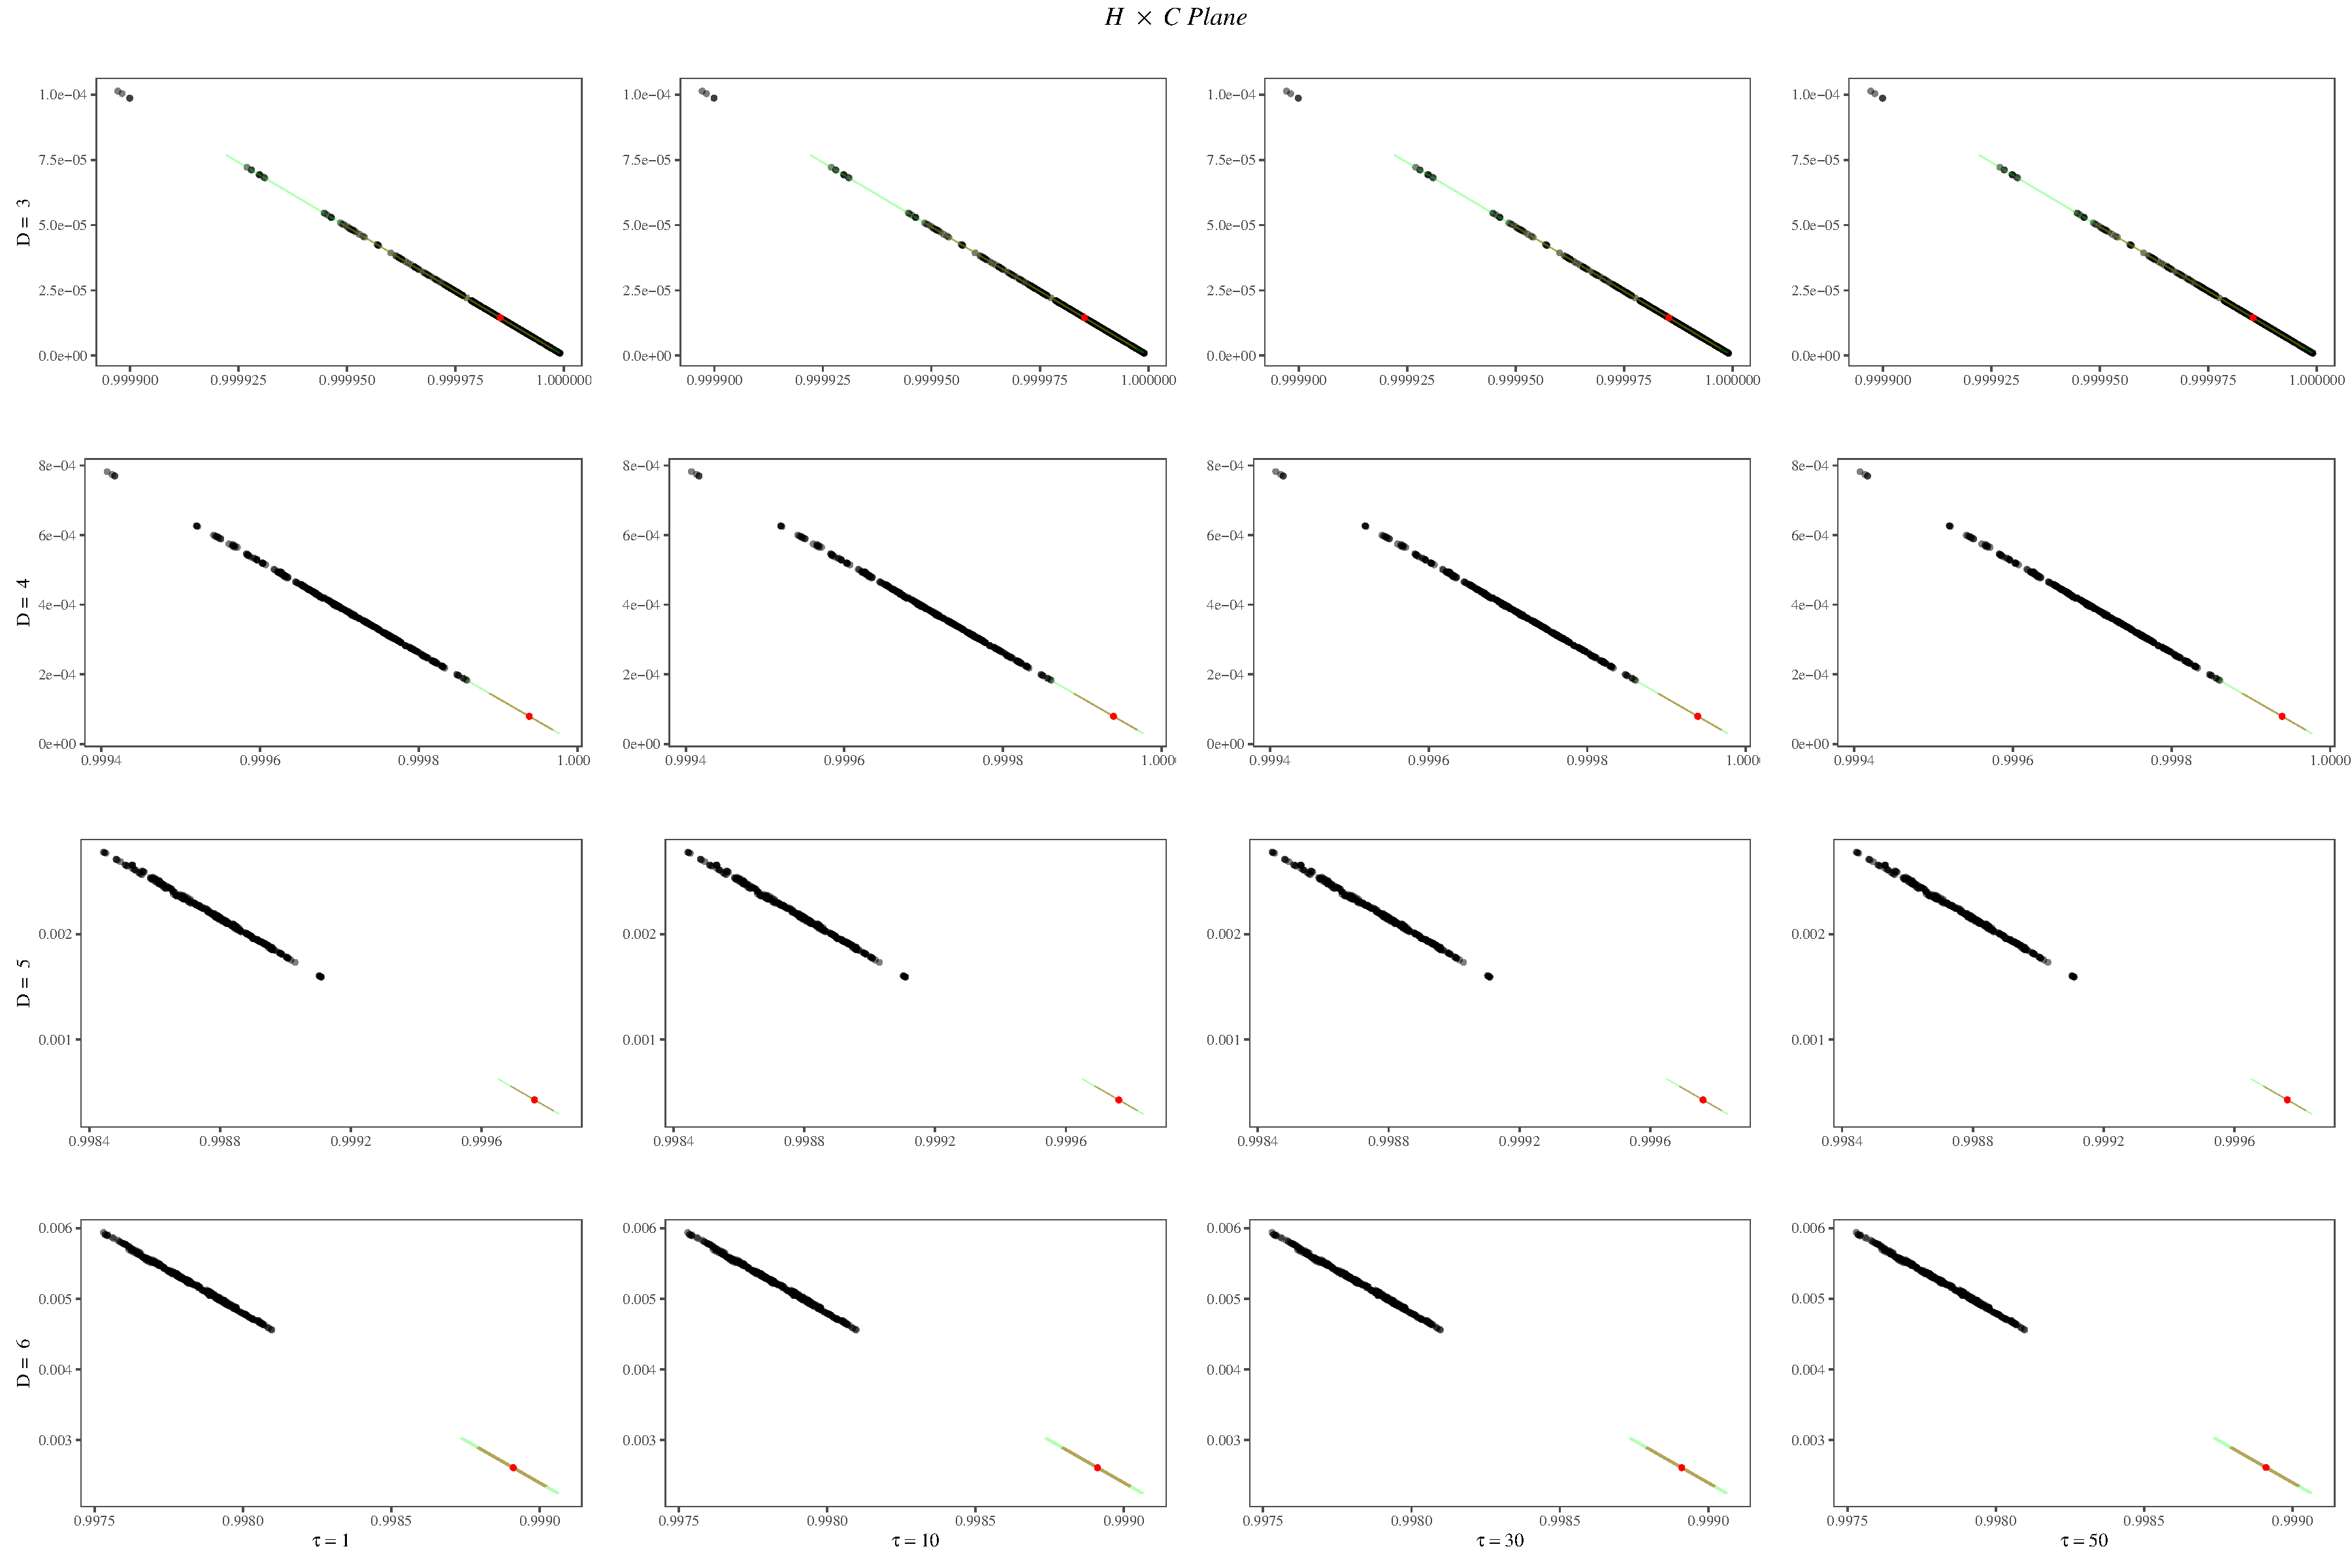
\includegraphics[width=\linewidth]{../../Images/PRNGs/Mersenne-50000.pdf}
	\caption{Scatter diagrams of the Mersenne-Twister sequences with 50.000 observations for D $\in \{3,4,5,6\}$ (columns) and $\tau \in \{1,10,30,50\}$ (lines).}
	\end{figure}

	\begin{figure}[H]
	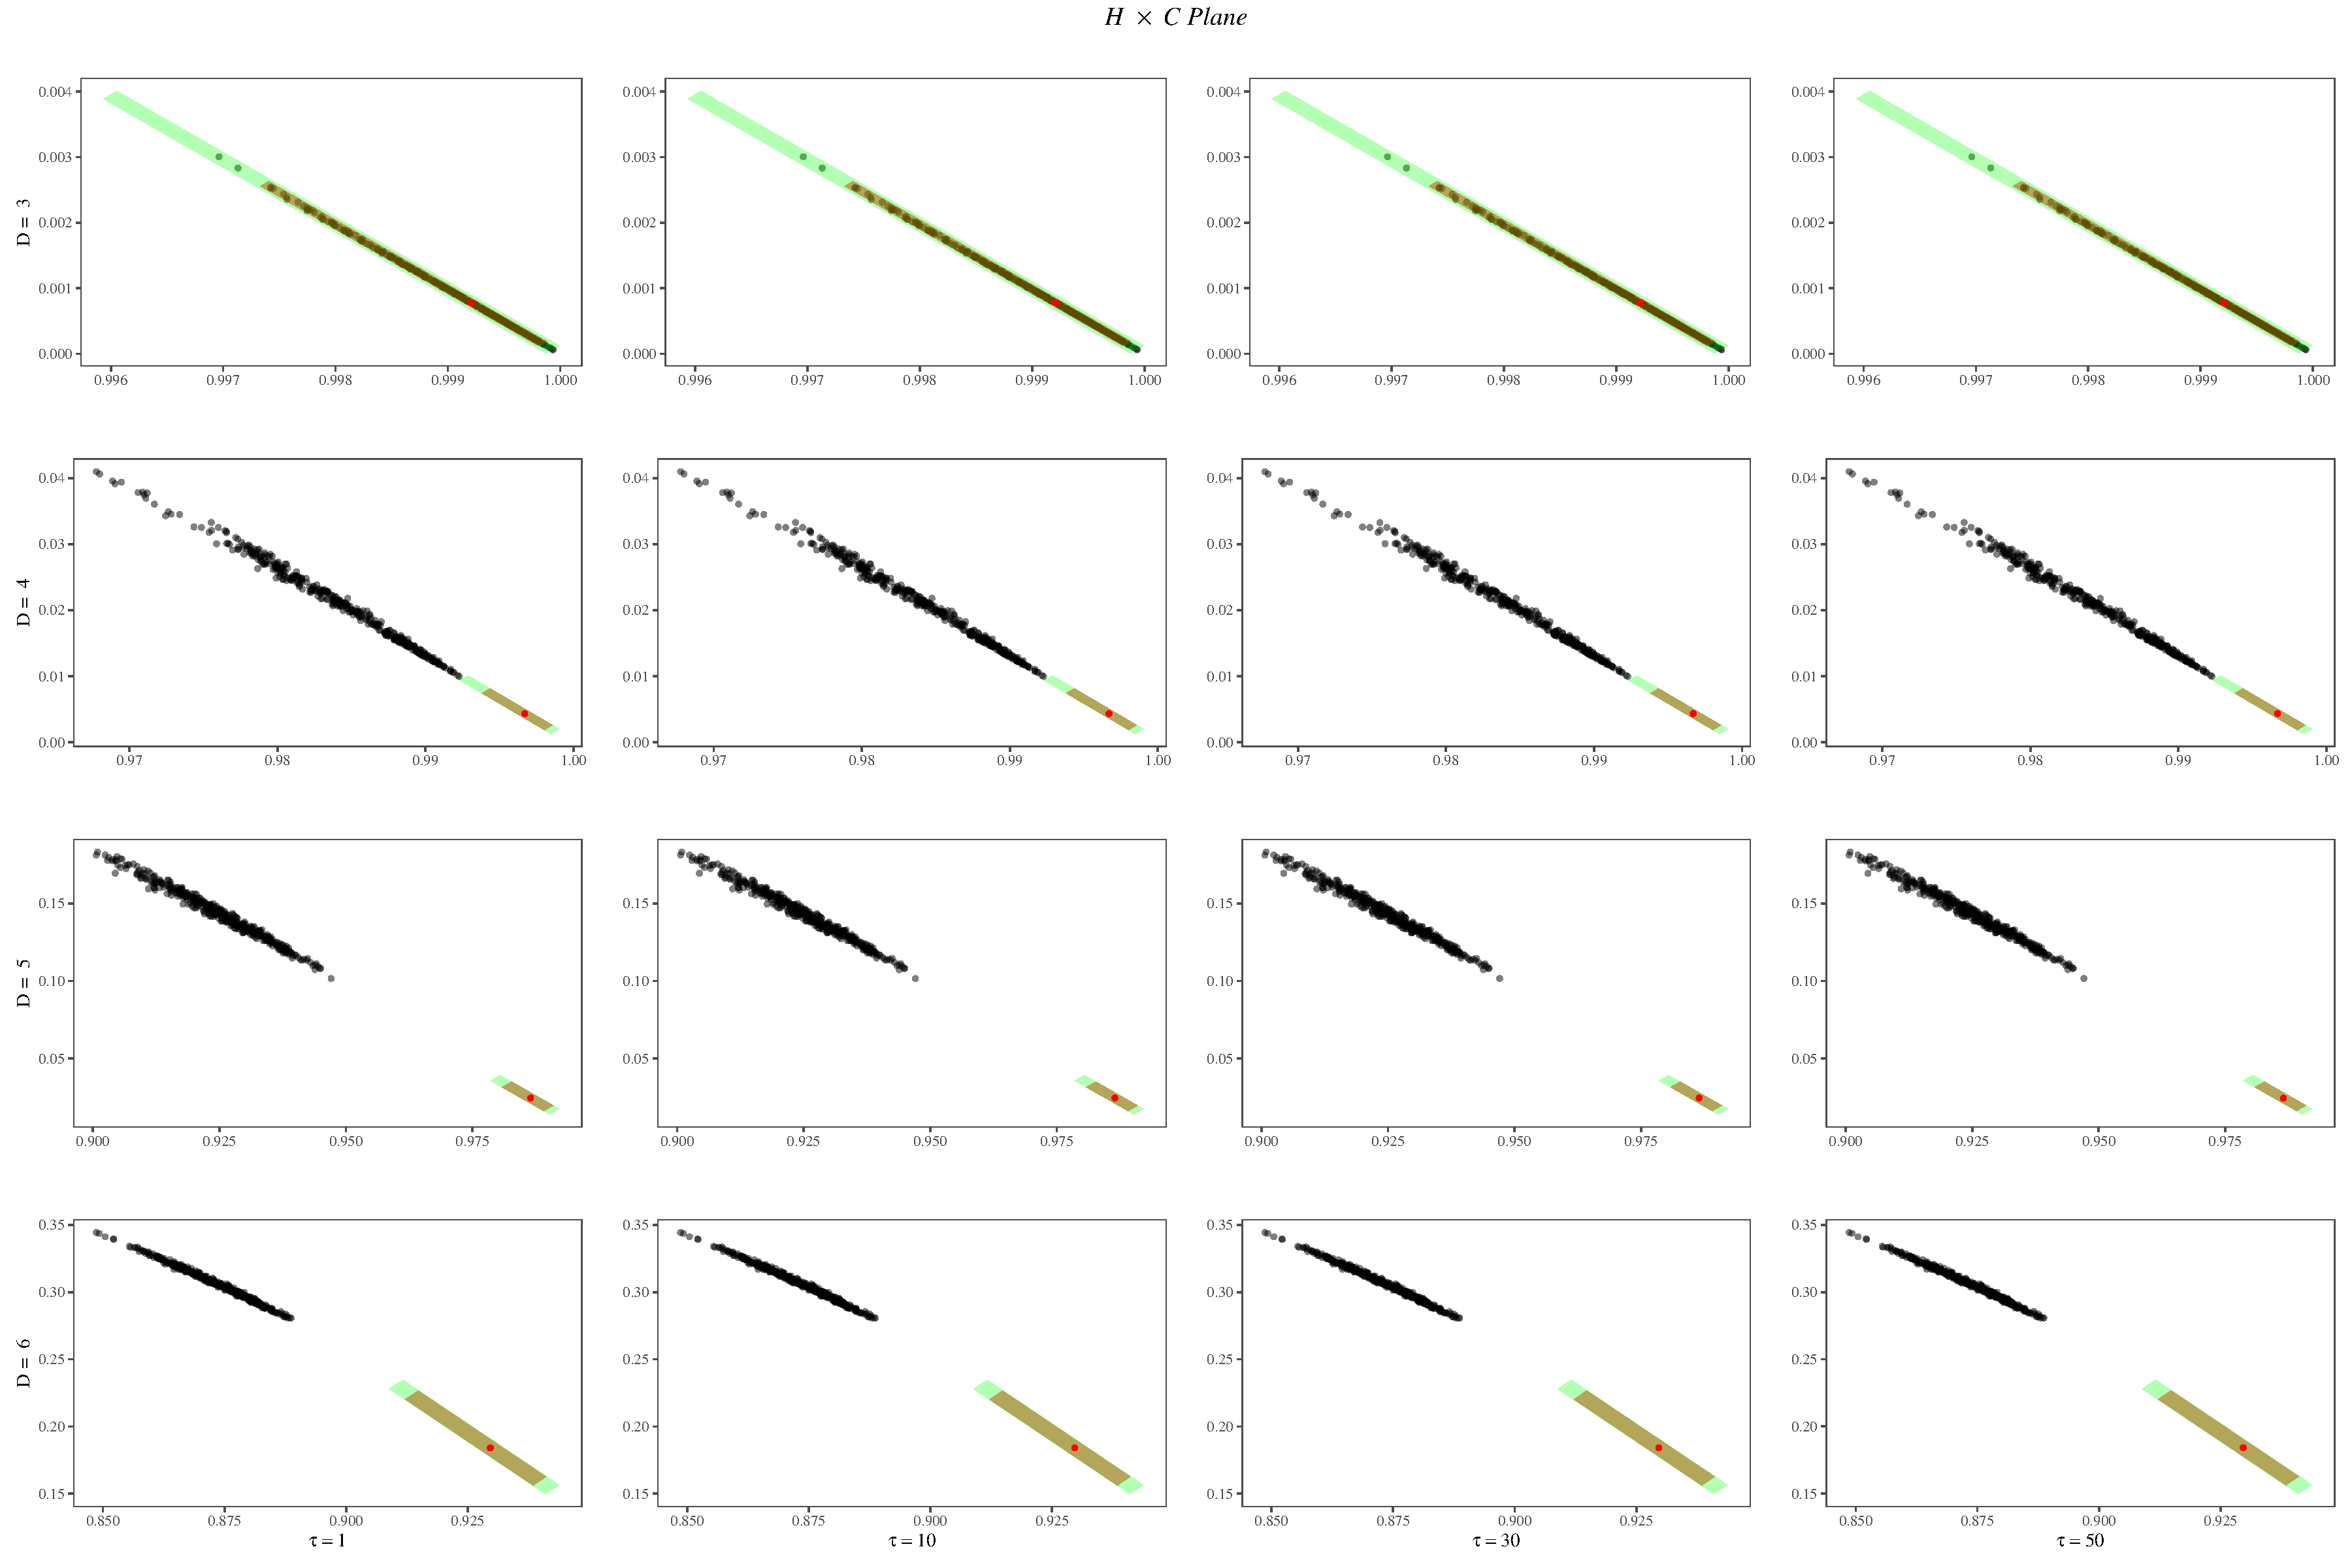
\includegraphics[width=\linewidth]{../../Images/PRNGs/N1000/Randu-1000.pdf}
	\caption{Scatter diagrams of the Randu sequences with 1.000 observations for D $\in \{3,4,5,6\}$ (columns) and $\tau \in \{1,10,30,50\}$ (lines).}
	\end{figure}

	\begin{figure}[H]
	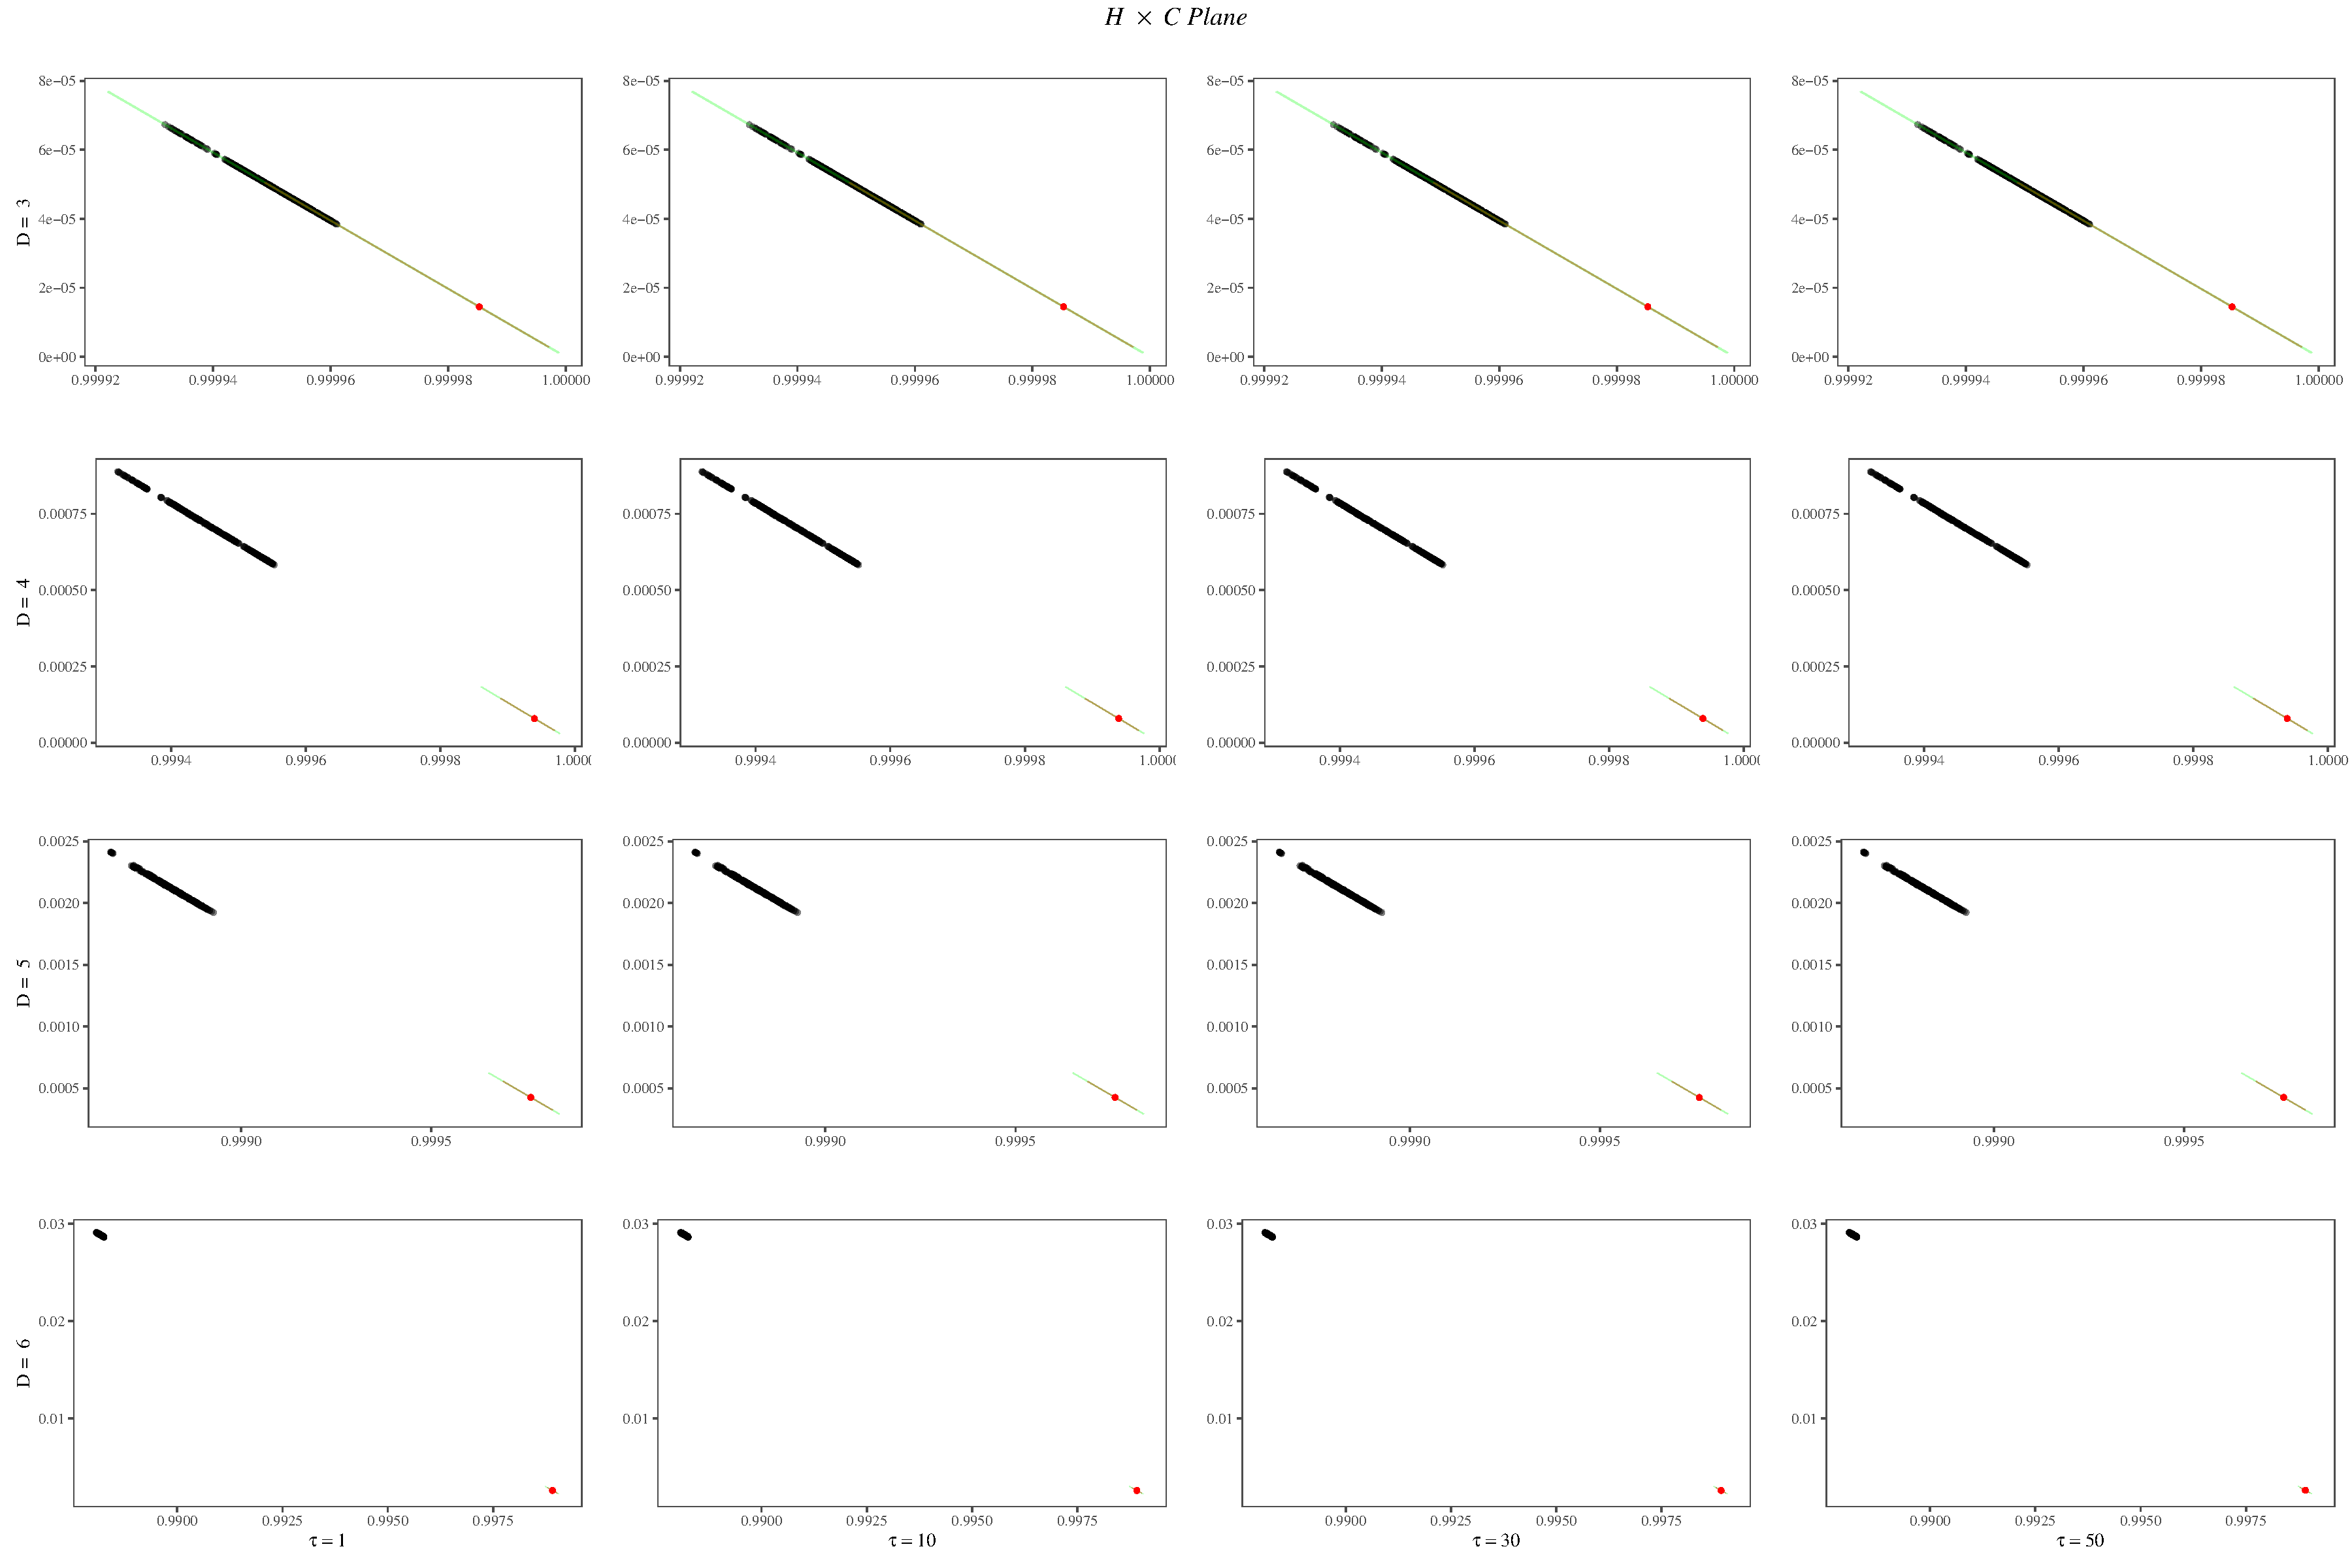
\includegraphics[width=\linewidth]{../../Images/PRNGs/Randu-50000.pdf}
	\caption{Scatter diagrams of the Randu sequences with 50.000 observations for D $\in \{3,4,5,6\}$ (columns) and $\tau \in \{1,10,30,50\}$ (lines).}
	\end{figure}
	\begin{table*}[!h]
	\centering
	\caption{Points inside the confidence regions}
	\label{tab:result1}
	\begin{tabular}{c*{5}r}
		\toprule
		Algorithm & \multicolumn{1}{c}{$N$} & \multicolumn{1}{c}{$D$} & \multicolumn{1}{c}{$\tau$} & \multicolumn{1}{c}{\SI{95}{\percent}} & \multicolumn{1}{c}{\SI{99}{\percent}}\\
		\cmidrule(lr){1-1}
		\cmidrule(lr){2-2}
		\cmidrule(lr){3-3}
		\cmidrule(lr){4-4}
		\cmidrule(lr){5-5}
		\cmidrule(lr){6-6}
		True-Random & 1000 & 3 & 1 & $91.0\%$ & $99.0\%$\\
		&  & 4 & 1 & $92.0\%$ & $98.0\%$\\
		&  & 5 & 1 & $88.0\%$ & $97.0\%$\\
		&  & 6 & 1 & $77.0\%$ & $96.0\%$\\
		\cmidrule(lr){1-6}
		True-Random & 50000 & 3 & 1 & $90.0\%$ & $97.0\%$\\
		&  & 4 & 1 & $89.0\%$ & $94.0\%$\\
		&  & 5 & 1 & $90.0\%$ & $96.0\%$\\
		&  & 6 & 1 & $88.0\%$ & $99.0\%$\\
		\cmidrule(lr){1-6}
		Mersenne-Twister & 1000 & 3 & 1 & $89.5\%$ & $97.5\%$\\
		 &  &  & 10 & $89.5\%$ & $97.5\%$\\
		 &  &  & 30 & $89.5\%$ & $97.5\%$\\
		 &  &  & 50 & $89.5\%$ & $97.5\%$\\
		\cmidrule(lr){1-6}
		Mersenne-Twister & 50000 & 3 & 1 & $91.0\%$ & $97.75\%$\\
		 &  &  & 10 & $89.5\%$ & $97.5\%$\\
		 &  &  & 30 & $89.5\%$ & $97.5\%$\\
		 &  &  & 50 & $89.5\%$ & $97.5\%$\\ \cmidrule(lr){3-6}
		 &  & 4 & 1 & $0.00\%$ & $0.25\%$\\
		 &  &  & 10 & $0.00\%$ & $0.25\%$\\
		 &  &  & 30 & $0.00\%$ & $0.25\%$\\
		 &  &  & 50 & $0.00\%$ & $0.25\%$\\
		\cmidrule(lr){1-6}
		Randu & 1000 & 3 & 1 & $97.25\%$ & $99.75\%$\\
		 &  & & 10 & $97.25\%$ & $99.75\%$\\
		 &  & & 30 & $97.25\%$ & $99.75\%$\\
		 &  & & 50 & $97.25\%$ & $99.75\%$\\
		\cmidrule(lr){1-6}
		Randu & 50000 & 3 & 1 & $53.0\%$ & $100.0\%$\\
		 &  &  & 10 & $53.0\%$ & $100.0\%$\\
		 &  &  & 30 & $53.0\%$ & $100.0\%$\\
		 &  &  & 50 & $53.0\%$ & $100.0\%$\\
		\bottomrule
	\end{tabular}
	\end{table*}

\begin{table*}[!h]
	\centering
	\caption{Points inside the confidence regions}
	\label{tab:result1}
	\begin{tabular}{c*{5}r}
		\toprule
		Algorithm & \multicolumn{1}{c}{$N$} & \multicolumn{1}{c}{$D$} & \multicolumn{1}{c}{$\tau$} & \multicolumn{1}{c}{\SI{95}{\percent}} & \multicolumn{1}{c}{\SI{99}{\percent}}\\
		\cmidrule(lr){1-1}
		\cmidrule(lr){2-2}
		\cmidrule(lr){3-3}
		\cmidrule(lr){4-4}
		\cmidrule(lr){5-5}
		\cmidrule(lr){6-6}
		Linear Congruential & 1000 & 3 & 1 & $92.0\%$ & $98.75\%$\\
		&  & & 10 & $92.0\%$ & $98.75\%$\\
		&  & & 30 & $92.0\%$ & $98.75\%$\\
		&  & & 50 & $92.0\%$ & $98.75\%$\\ 
		\cmidrule(lr){3-6}
		&  & 4 & 1 & $0.00\%$ & $0.5\%$\\
		&  &   & 10& $0.00\%$ & $0.5\%$\\
		&  &  & 30 & $0.00\%$ & $0.5\%$\\
		&  &  & 50 & $0.00\%$ & $0.5\%$\\
		\cmidrule(lr){1-6}
		Linear Congruential & 50000 & 3 & 1 & $12.0\%$ & $16.0\%$\\
		&  & & 10 & $12.0\%$ & $16.0\%$\\
		&  & & 30 & $12.0\%$ & $16.0\%$\\
		&  & & 50 & $12.0\%$ & $16.0\%$\\ 
		\bottomrule
	\end{tabular}
\end{table*}

\begin{table*}[!h]
\centering
\caption{Points inside the confidence regions}
\label{tab:result1}
\begin{tabular}{c*{5}r}
	\toprule
	Algorithm & \multicolumn{1}{c}{$N$} & \multicolumn{1}{c}{$D$} & \multicolumn{1}{c}{$\tau$} & \multicolumn{1}{c}{\SI{95}{\percent}} & \multicolumn{1}{c}{\SI{99}{\percent}}\\
	\cmidrule(lr){1-1}
	\cmidrule(lr){2-2}
	\cmidrule(lr){3-3}
	\cmidrule(lr){4-4}
	\cmidrule(lr){5-5}
	\cmidrule(lr){6-6}
	Wichmann-Hill & 50000 & 3 & 1 & $87.5\%$ & $98.75\%$\\
	&  & & 10 & $87.5\%$ & $98.75\%$\\
	&  & & 30 & $87.5\%$ & $98.75\%$\\
	&  & & 50 & $87.5\%$ & $98.75\%$\\ 
	\cmidrule(lr){3-6}
	&  & 4 & 1 & $0.00\%$ & $1.0\%$\\
	&  &   & 10& $0.00\%$ & $1.0\%$\\
	&  &  & 30 & $0.00\%$ & $1.0\%$\\
	&  &  & 50 & $0.00\%$ & $1.0\%$\\
	\cmidrule(lr){1-6}
	Marsaglia-Multicarry & 50000 & 3 & 1 & $91.25\%$ & $98.00\%$\\
	&  & & 10 & $91.25\%$ & $98.00\%$\\
	&  & & 30 & $91.25\%$ & $98.00\%$\\
	&  & & 50 & $91.25\%$ & $98.00\%$\\ 
	\cmidrule(lr){3-6}
	&  & 4 & 1 & $0.00\%$ & $2.0\%$\\
	&  &   & 10& $0.00\%$ & $2.0\%$\\
	&  &  & 30 & $0.00\%$ & $2.0\%$\\
	&  &  & 50 & $0.00\%$ & $2.0\%$\\
	\cmidrule(lr){1-6}
	Super-Duper & 50000 & 3 & 1 & $92.00\%$ & $98.00\%$\\
	&  & & 10 & $92.00\%$ & $98.00\%.$\\
	&  & & 30 & $92.00\%$ & $98.00\%$\\
	&  & & 50 & $92.00\%$ & $98.00\%$\\ 
	\cmidrule(lr){3-6}
	&  & 4 & 1 & $0.00\%$ & $0.50\%$\\
	&  &   & 10& $0.00\%$ & $0.50\%$\\
	&  &  & 30 & $0.00\%$ & $0.50\%$\\
	&  &  & 50 & $0.00\%$ & $0.50\%$\\
	\cmidrule(lr){1-6}
	Knuth-TAOCP-2002 & 50000 & 3 & 1 & $89.25\%$ & $96.5\%$\\
	&  & & 10 & $89.25\%$ & $96.5\%.$\\
	&  & & 30 & $89.25\%$ & $96.5\%$\\
	&  & & 50 & $89.25\%$ & $96.5\%$\\ 
	\cmidrule(lr){1-6}
	Knuth-TAOCP & 50000 & 3 & 1 & $93.75\%$ & $99.00\%$\\
	&  & & 10 & $93.75\%$ & $99.00\%.$\\
	&  & & 30 & $93.75\%$ & $99.00\%$\\
	&  & & 50 & $93.75\%$ & $99.00\%$\\ 
	\cmidrule(lr){3-6}
	&  & 4 & 1 & $0.00\%$ & $1.00\%$\\
	&  &   & 10& $0.00\%$ & $1.00\%$\\
	&  &  & 30 & $0.00\%$ & $1.00\%$\\
	&  &  & 50 & $0.00\%$ & $1.00\%$\\
	\cmidrule(lr){1-6}
	\bottomrule
\end{tabular}
\end{table*}

\begin{table*}[!h]
	\centering
	\caption{Points inside the confidence regions}
	\label{tab:result1}
	\begin{tabular}{c*{5}r}
		\toprule
		Algorithm & \multicolumn{1}{c}{$N$} & \multicolumn{1}{c}{$D$} & \multicolumn{1}{c}{$\tau$} & \multicolumn{1}{c}{\SI{95}{\percent}} & \multicolumn{1}{c}{\SI{99}{\percent}}\\
		\cmidrule(lr){1-1}
		\cmidrule(lr){2-2}
		\cmidrule(lr){3-3}
		\cmidrule(lr){4-4}
		\cmidrule(lr){5-5}
		\cmidrule(lr){6-6}
		L'Ecuyer-CMRG & 50000 & 3 & 1 & $92.25 \%$ & $98.00\%$\\
		&  & & 10 & $92.25\%$ & $98.00\%.$\\
		&  & & 30 & $92.25\%$ & $98.00\%$\\
		&  & & 50 & $92.25\%$ & $98.00\%$\\ 
		\cmidrule(lr){3-6}
		&  & 4 & 1 & $0.00\%$ & $1.00\%$\\
		&  &   & 10& $0.00\%$ & $1.00\%$\\
		&  &  & 30 & $0.00\%$ & $1.00\%$\\
		&  &  & 50 & $0.00\%$ & $1.00\%$\\
		\cmidrule(lr){1-6}
		\bottomrule
	\end{tabular}
\end{table*}

\begin{table*}[!h]
\centering
\caption{Points inside the confidence regions}
\label{tab:result1}
\begin{tabular}{c*{5}r}
	\toprule
	Algorithm & \multicolumn{1}{c}{$N$} & \multicolumn{1}{c}{$D$} & \multicolumn{1}{c}{$\tau$} & \multicolumn{1}{c}{\SI{95}{\percent}} & \multicolumn{1}{c}{\SI{99}{\percent}}\\
	\cmidrule(lr){1-1}
	\cmidrule(lr){2-2}
	\cmidrule(lr){3-3}
	\cmidrule(lr){4-4}
	\cmidrule(lr){5-5}
	\cmidrule(lr){6-6}
	pcg64 & 50000 & 3 & 1 & $87.50 \%$ & $96.00\%$\\
	&  & & 10 & $87.50\%$ & $96.00\%.$\\
	&  & & 30 & $87.50\%$ & $96.00\%$\\
	&  & & 50 & $87.50\%$ & $96.00\%$\\ 
	\cmidrule(lr){3-6}
	&  & 4 & 1 & $0.00\%$ & $1.00\%$\\
	&  &   & 10& $0.00\%$ & $1.00\%$\\
	&  &  & 30 & $0.00\%$ & $1.00\%$\\
	&  &  & 50 & $0.00\%$ & $1.00\%$\\
	\cmidrule(lr){1-6}
	Xoroshiro128+ & 50000 & 3 & 1 & $92.25 \%$ & $98.00\%$\\
	&  & & 10 & $92.25\%$ & $98.00\%.$\\
	&  & & 30 & $92.25\%$ & $98.00\%$\\
	&  & & 50 & $92.25\%$ & $98.00\%$\\ 
	\cmidrule(lr){3-6}
	&  & 4 & 1 & $2.00\%$ & $3.00\%$\\
	&  &   & 10& $2.00\%$ & $3.00\%$\\
	&  &  & 30 & $2.00\%$ & $3.00\%$\\
	&  &  & 50 & $2.00\%$ & $3.00\%$\\
	\cmidrule(lr){1-6}
	Xoshiro256+ & 50000 & 3 & 1 & $83.75 \%$ & $96.00\%$\\
	&  & & 10 & $83.75\%$ & $96.00\%.$\\
	&  & & 30 & $83.75\%$ & $96.00\%$\\
	&  & & 50 & $83.75\%$ & $96.00\%$\\ 
	\cmidrule(lr){3-6}
	&  & 4 & 1 & $2.00\%$ & $3.00\%$\\
	&  &   & 10& $2.00\%$ & $3.00\%$\\
	&  &  & 30 & $2.00\%$ & $3.00\%$\\
	&  &  & 50 & $2.00\%$ & $3.00\%$\\
	\cmidrule(lr){1-6}
	Threefry & 50000 & 3 & 1 & $87.25 \%$ & $97.50\%$\\
	&  & & 10 & $87.25\%$ & $97.50\%.$\\
	&  & & 30 & $87.25\%$ & $97.50\%$\\
	&  & & 50 & $87.25\%$ & $97.50\%$\\ 
	\cmidrule(lr){3-6}
	&  & 4 & 1 & $0.00\%$ & $3.50\%$\\
	&  &   & 10& $0.00\%$ & $3.50\%$\\
	&  &  & 30 & $0.00\%$ & $3.50\%$\\
	&  &  & 50 & $0.00\%$ & $3.50\%$\\
	\cmidrule(lr){1-6}
	\bottomrule
\end{tabular}
\end{table*}
\end{description}
 
\end{document}
